\subsubsection{UC6.4 - Personalizzazione Proiezione Lineare Multi Asse}
\begin{figure}[h]
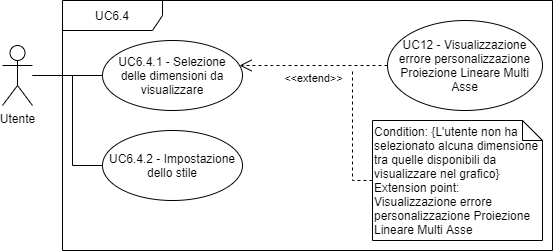
\includegraphics[width=\linewidth]{Section/Images/UC6.4.png}
\centering
\caption{UC6.4 - Personalizzazione Proiezione Lineare Multi Asse}
\end{figure}
\begin{itemize}
	\item \textbf{Attore primario}: Utente.
	
	\item \textbf{Precondizioni}: L'utente ha scelto il grafico \textit{Proiezione Lineare Multi Asse} [UC5.4].
	
	\item \textbf{Postcondizioni}: Il grafico viene aggiornato.
	
	\item \textbf{Scenario principale}: L'utente decide:
	
\begin{enumerate}
\item Le dimensioni da visualizzare [UC6.4.1];
\item Alcuni stili del grafico [UC6.4.2].
\end{enumerate}	
		
\end{itemize}